\chapter{झिल्ली यातायात और प्रोटीन छँटाई}\label{ch:b3:membrane-traffic}

अग्न्याशय की कोई कोशिका हर मिनट पाचक एंज़ाइम के कोई एक करोड़ अणु बनाती
है, उन्हें कणिकाओं में भरती है, और आँत के किसी संकेत पर उन्हें किसी
वाहिनी में छोड़ देती है --- और अपने ही कोशिकाद्रव्य में ट्रिप्सिन का एक
अणु भी कभी खुला नहीं छोड़ती। यकृत की कोई कोशिका रक्त से कोलेस्टेरॉल
निकालती है, उसे ढोने वाले कणों को पूरा-का-पूरा निगलकर, हर मिनट हज़ारों
की दर से, और हर ग्राही अगली बार के लिए पृष्ठ पर लौटा देती है।
सूत्रकणिका, केंद्रक, \omterm{def:b3:membrane-traffic:endocytosis}{लयनकाय}, झिल्ली या बाहरी संसार के लिए नियत कोई
नया बना प्रोटीन दर्जन भर कक्षों के बीच अपने पते तक ऐसी त्रुटि-दर के साथ
पहुँचता है जो किसी डाक-सेवा को लज्जित कर दे। यह अध्याय उसी छँटाई के
बारे में है: प्रोटीनों में लिखे संकेत, उन्हें पढ़ने वाली मशीनें, वे
पुटिकाएँ जो कक्षों के बीच झिल्ली और भार ढोती हैं, वे \omterm{def:b3:membrane-traffic:coats}{आवरण} जो पुटिकाओं
को आकार देते हैं और वे प्रोटीन जो उन्हें सही लक्ष्य से संलयित कराते
हैं, और वह दोतरफ़ा यातायात --- बाहर स्राव, भीतर अंतर्ग्रहण --- जो कोई
सुकेंद्रकी कोशिका अपने जीवन के हर सेकंड चलाए रखती है।

\section{संकेत और पते}

\begin{definition}[छँटाई संकेत]\label{def:b3:membrane-traffic:signals}
\index{छँटाई संकेत}\index{संकेत पेप्टाइड}\index{केंद्रक-स्थानिकीकरण संकेत}\index{पूर्वानुक्रम}
कोई \emph{छँटाई संकेत} किसी प्रोटीन का कोई खंड, या उसका कोई रूपांतरण
है, जिसे कोई ग्राही पढ़कर प्रोटीन को किसी एक कक्ष तक पहुँचा देता है।
\emph{संकेत पेप्टाइड}, यानी अमीनो सिरे पर जलविरोधी क्रोड वाला
\numrange{15}{30} अवशेषों का कोई खंड, किसी प्रोटीन को बनते-बनते ही
अंतर्द्रव्यी जालिका में भेज देता है; वहाँ से चूक-मार्ग गॉल्जी से होकर
जीवद्रव्य-कला तक या बाहर तक जाता है, और आगे के संकेत उसे \omterm{def:b3:membrane-traffic:endocytosis}{लयनकाय} की ओर
(कोई फ़ॉस्फ़ोरिलित शर्करा) या जालिका में वापस (कार्बोक्सी-सिरे का
अनुक्रम KDEL) मोड़ देते हैं। कोई
\emph{केंद्रक-स्थानिकीकरण संकेत}, यानी PKKKRKV जैसा कोई छोटा क्षारीय
टुकड़ा, इंपोर्टिनों से बँधता है जो वलित प्रोटीन को केंद्रक-छिद्र से पार
ले जाते हैं; कोई सूत्रकणिकीय \emph{पूर्वानुक्रम}, यानी
\numrange{20}{50} अवशेषों की कोई उभयरागी कुंडली, बाहरी झिल्ली के
ग्राहियों से पहचाना जाता है और दोनों झिल्लियों के स्थानांतरकों से,
अवलित, पिरो दिया जाता है; परऑक्सीकायी एंज़ाइमों का अंत SKL पर होता है।
जिन प्रोटीनों में इनमें से कुछ नहीं होता वे कोशिकाद्रव्य में रह जाते
हैं। हर संकेत उसी एक ढंग से मिला: उसे हटा दीजिए तो प्रोटीन
कोशिकाद्रव्य में रह जाता है, उसे किसी कोशिकाद्रव्यी प्रोटीन पर जोड़
दीजिए तो वह प्रोटीन उस कक्ष में चला जाता है।
\end{definition}

\begin{proof}[प्रमाण-सामग्री]
ब्लोबेल और डॉबरश्टाइन (1975) ने किसी प्रतिरक्षी लघु शृंखला के संदेशवाहक
RNA का अनुवादन किसी कोशिका-मुक्त तंत्र में किया। बिना झिल्लियों के
उत्पाद स्रावित प्रोटीन से लगभग बीस अवशेष लंबा था;
अनुवादन के \emph{दौरान} अंतर्द्रव्यी जालिका के टुकड़े जोड़ देने पर
उत्पाद स्रावित आकार का था और जोड़े गए प्रोटिएज़ से सुरक्षित था ---
वह पुटिकाओं के भीतर था --- जबकि अनुवादन के बाद जोड़ी गई झिल्लियों ने
कुछ नहीं किया। अतिरिक्त अमीनो-सिरे वाला खंड, यानी \omterm{def:b3:membrane-traffic:signals}{संकेत पेप्टाइड},
जालिका में घुसने के लिए चाहिए, उसके भीतर हटा दिया जाता है, और केवल तभी
काम करता है जब शृंखला बन रही हो: यही \emph{संकेत
परिकल्पना} है, जिसकी हर विवरण में पुष्टि तब हुई जब ग्राही
(संकेत-पहचान कण, वॉल्टर और ब्लोबेल 1981) और वाहिका
(Sec61) शुद्ध किए गए।
\end{proof}

\begin{omfigure}
\begin{tikzpicture}[every node/.style={font=\scriptsize}, >=stealth]
  % ER membrane
  \fill[omDef!15] (0,0) rectangle (12,-1.6);
  \draw[very thick, omDef] (0,0) -- (12,0); \draw[very thick, omDef] (0,-0.35) -- (12,-0.35);
  \node[right, omDef!70!black] at (0.1,-1.3) {ER अवकाशिका};
  \node[right] at (0.1,2.9) {कोशिकाद्रव्य};
  % stage 1: ribosome with emerging signal peptide + SRP
  \draw[thick, fill=gray!25] (1.4,1.6) circle (0.5); \draw[thick, fill=gray!25] (1.4,0.95) ellipse (0.62 and 0.3);
  \draw[very thick, omThm] (1.4,0.65) -- (1.4,0.2) -- (1.9,0.1);
  \draw[thick, fill=omProp!40] (2.1,0.35) ellipse (0.35 and 0.2); \node[above right] at (2.2,0.5) {SRP};
  \node[below, align=center] at (1.7,-1.7) {1. संकेत पेप्टाइड निकलता है;\\SRP बँधता है, अनुवादन रुकता है};
  % stage 2: docking at SRP receptor and translocon
  \draw[->, thick] (3.2,1.2) -- (4.2,1.2);
  \draw[thick, fill=gray!25] (5.6,1.75) circle (0.5); \draw[thick, fill=gray!25] (5.6,1.1) ellipse (0.62 and 0.3);
  \draw[thick, fill=omMeth!40] (5.2,0.0) rectangle (5.45,-0.35); \draw[thick, fill=omMeth!40] (5.75,0.0) rectangle (6.0,-0.35);
  \node[below, align=center] at (5.9,-1.7) {2. SRP ग्राही उसे Sec61 पर\\जोड़ता है; SRP चला जाता है};
  \draw[very thick, omThm] (5.6,0.8) -- (5.6,-0.2);
  \draw[thick, fill=omProp!40] (4.7,0.15) ellipse (0.3 and 0.18); \node[above] at (4.7,0.33) {SRP ग्राही};
  % stage 3: translocation, cleavage, glycosylation
  \draw[->, thick] (7.2,1.2) -- (8.2,1.2);
  \draw[thick, fill=gray!25] (9.6,1.75) circle (0.5); \draw[thick, fill=gray!25] (9.6,1.1) ellipse (0.62 and 0.3);
  \draw[thick, fill=omMeth!40] (9.2,0.0) rectangle (9.45,-0.35); \draw[thick, fill=omMeth!40] (9.75,0.0) rectangle (10.0,-0.35);
  \draw[very thick, omThm] (9.6,0.8) -- (9.6,-0.5) .. controls (9.6,-1.0) and (10.3,-1.1) .. (10.6,-0.7);
  \draw[omThm, thick] (10.9,-0.9) -- (11.2,-0.9); \node[right, font=\tiny] at (11.0,-1.15) {संकेत कटा};
  \fill[omExo] (10.3,-1.0) circle (0.07); \fill[omExo] (10.45,-1.12) circle (0.07); \node[below, font=\tiny] at (10.2,-1.15) {शर्कराएँ};
  \node[below, align=center] at (10.0,-1.7) {3. शृंखला बनते-बनते पार करती है;\\संकेत कटा, शर्कराएँ जुड़ीं};
\end{tikzpicture}

{\small संकेत परिकल्पना। नवजात शृंखला के आरंभ पर पड़े \omterm{def:b3:membrane-traffic:signals}{संकेत पेप्टाइड} से
संकेत-पहचान कण बँधता है, जो अनुवादन रोक देता है और राइबोसोम को Sec61
वाहिका पर जोड़ देता है; फिर शृंखला संश्लेषित होते-होते झिल्ली पार कर
जाती है, संकेत अवकाशिका में काट दिया जाता है, और शर्कराएँ जोड़ी जाती
हैं।}
\end{omfigure}

\begin{proposition}[झिल्ली प्रोटीन और सांस्थिति]\label{prop:b3:membrane-traffic:topology}
\index{विराम-स्थानांतरण अनुक्रम}\index{झिल्ली सांस्थिति}
स्थानांतरित हो रही किसी शृंखला के बीच में पड़ा लगभग बीस अवशेषों का कोई
जलविरोधी खंड \emph{विराम-स्थानांतरण} अनुक्रम का काम करता है: वाहिका
बगल से खुलती है और उसे द्विपरत में किसी झिल्ली-पारी कुंडली के रूप में
छोड़ देती है, जिसमें पहले से स्थानांतरित भाग अवकाशिका में रहता है और
शेष कोशिकाद्रव्य में बनता है। ऐसा दूसरा खंड स्थानांतरण फिर चालू कर देता
है, और $n$ बारी-बारी के संकेतों वाला कोई प्रोटीन
$n$ झिल्ली-पारी कुंडलियों के साथ समाप्त होता है। जालिका में तय हुई दिशा
कभी नहीं बदलती: जो जालिका की अवकाशिका की ओर है वह गॉल्जी की और उसके बाद
हर पुटिका की अवकाशिका की ओर रहता है, और जीवद्रव्य-कला से संलयन के बाद
कोशिका के \emph{बाहर} की ओर। इसलिए शर्कराएँ, जो केवल अवकाशिका में जुड़ती
हैं, किसी पृष्ठ-प्रोटीन के सदा बाह्यकोशिकीय फलक पर होती हैं, और किसी
ग्राही की सांस्थिति इसी से पढ़ी जा सकती है कि उसके ग्लाइकोसिलन-स्थल
कहाँ पड़े हैं।
\end{proposition}

\begin{method}[स्फुरण--अनुधावन]\label{met:b3:membrane-traffic:pulse-chase}
\index{स्फुरण--अनुधावन}\index{स्वविकिरणचित्रण}
नए बने अणुओं की किसी समष्टि का कोशिका भर पीछा करने के लिए: (1)
कोशिकाओं को थोड़ी देर (\emph{स्फुरण}, कुछ मिनट) किसी रेडियोधर्मी या
अन्यथा अंकित पूर्वगामी के संपर्क में लाइए --- प्रोटीनों के लिए
ट्रिटियमित ल्यूसीन; (2) उसे बिना अंकित पूर्वगामी की अधिकता से बदल
दीजिए (\emph{अनुधावन}), ताकि कोई नया चिह्न न जुड़े; (3) अंतरालों पर
कोशिकाओं के प्रतिदर्श स्थिर कीजिए और चिह्न को इलेक्ट्रॉन
सूक्ष्मचित्रों में स्वविकिरणचित्रण से, या कक्षों को अलग करके गिनकर,
ढूँढ़िए; (4) हर कक्ष में चिह्न का अंश समय के सामने आलेखित कीजिए। जिस
क्रम में कक्ष भरते और खाली होते हैं वही मार्ग है; समय-निर्धारण हर कक्ष
में निवास-काल देता है। पैलेड की प्रयोगशाला (1960 के दशक) ने इसे
अग्न्याशय की कूपिका-कोशिका पर लगाया और चिह्न को \qty{3}{min} पर खुरदरी
जालिका में, \qty{20}{min} पर गॉल्जी में, \qty{40}{min} पर संघनक
रसधानियों तथा कणिकाओं में, और एक घंटे बाद तथा किसी संकेत पर वाहिनी में
पाया: स्रावी पथ, समय में बिछा हुआ।
\end{method}

\begin{theorem}[क्रमिक कक्ष और स्फुरण--अनुधावन वक्र]\label{thm:b3:membrane-traffic:pulse-chase}
\index{कक्ष प्रतिरूप}
मान लीजिए अंकित प्रोटीन का कोई स्फुरण कक्ष $A$ से $B$ की ओर
प्रथम-कोटि दर $k_{1}$ से जाता है और $B$ से $C$ की ओर दर $k_{2}$ से, और
$C$ उसे रोक लेता है। सारा चिह्न $A$ में हो, $t = 0$ पर, तो
\[
A(t) = e^{-k_{1}t},\qquad
B(t) = \frac{k_{1}}{k_{2} - k_{1}}\bigl(e^{-k_{1}t} - e^{-k_{2}t}\bigr),
\qquad
C(t) = 1 - A - B,
\]
और $B$ में चिह्न $t^{*} = \ln(k_{2}/k_{1})/(k_{2} - k_{1})$ पर शिखर छूता है।
$A$ में माध्य निवास-काल $1/k_{1}$ है और $B$ में $1/k_{2}$,
चाहे दोनों दरों का क्रम कुछ भी हो।
\end{theorem}
\begin{proof}
$\mathrm{d}A/\mathrm{d}t = -k_{1}A$ से चरघातांकी रूप मिलता है। $B$ के लिए
$\mathrm{d}B/\mathrm{d}t = k_{1}A - k_{2}B = k_{1}e^{-k_{1}t} - k_{2}B$;
$B = \beta(e^{-k_{1}t} - e^{-k_{2}t})$ आज़माइए: अवकलज
$\beta(-k_{1}e^{-k_{1}t} + k_{2}e^{-k_{2}t})$ है और $-k_{2}B = \beta(-k_{2}
e^{-k_{1}t} + k_{2}e^{-k_{2}t})$, इसलिए समीकरण को $\beta(k_{2}
- k_{1})e^{-k_{1}t} = k_{1}e^{-k_{1}t}$ चाहिए, यानी $\beta = k_{1}/(k_{2} -
k_{1})$, और $B(0) = 0$ भी, जैसा चाहिए। $\mathrm{d}B/\mathrm{d}t =
0$ रखने पर $k_{1}e^{-k_{1}t} = k_{2}e^{-k_{2}t}$, जिससे $t^{*}$ मिलता
है। दर $k$ से छोड़े जाने वाले किसी कक्ष में कोई अणु माध्य $\int_{0}^{
\infty} t\,k e^{-kt}\,\mathrm{d}t = 1/k$ समय बिताता है।
\end{proof}

\begin{example}[संख्याओं में पैलेड की कोशिका]\label{ex:b3:membrane-traffic:palade}
$k_{1} = \qty{0.1}{min^{-1}}$ (जालिका में दस मिनट) और
$k_{2} = \qty{0.05}{min^{-1}}$ (गॉल्जी में बीस) लीजिए। गॉल्जी
$t^{*} = \ln 2/0.05 = \qty{13.9}{min}$ पर शिखर छूता है और तब $B = 2(e^{-1.39} -
e^{-0.69}) = 2(0.25 - 0.50)\cdot(-1) = 0.50$ रखता है: चिह्न का आधा।
\qty{40}{min} पर $A = 0.018$, $B = 2(0.018 - 0.135) \to 0.23$, $C = 0.75$:
प्रोटीन का तीन-चौथाई कणिकाओं तक पहुँच चुका है। पैलेड की प्रयोगशाला के
प्रेक्षित वक्रों का यही आकार है, और उन्हें फिट करना ही वह ढंग था जिससे
निवास-काल पहली बार मापे गए।
\end{example}

\begin{omfigure}
\begin{tikzpicture}
\begin{axis}[
  width=0.7\linewidth, height=5.6cm,
  axis x line=bottom, axis y line=left,
  xmin=0, xmax=80, ymin=0, ymax=1.05,
  xlabel={स्फुरण के बाद के मिनट}, ylabel={चिह्न का अंश},
  xlabel style={font=\small, at={(axis description cs:0.5,-0.12)}, anchor=north},
  ylabel style={font=\small},
  tick label style={font=\small}, xtick={0,20,40,60,80}, ytick={0,0.5,1},
  clip=false,
]
\addplot[very thick, omDef, domain=0:80, samples=80] {exp(-0.1*x)};
\addplot[very thick, omProp, domain=0:80, samples=80] {2*(exp(-0.05*x)-exp(-0.1*x))};
\addplot[very thick, omMeth!70!black, domain=0:80, samples=80] {1-exp(-0.1*x)-2*(exp(-0.05*x)-exp(-0.1*x))};
\node[font=\scriptsize, omDef, anchor=south west] at (axis cs:4,0.62) {जालिका, $A$};
\node[font=\scriptsize, omProp, anchor=south] at (axis cs:14,0.53) {गॉल्जी, $B$};
\node[font=\scriptsize, omMeth!70!black, anchor=north west] at (axis cs:45,0.72) {कणिकाएँ, $C$};
\end{axis}
\end{tikzpicture}

{\small $k_{1} =
\qty{0.1}{min^{-1}}$ और $k_{2} = \qty{0.05}{min^{-1}}$ वाले दो-दर
प्रतिरूप से स्फुरण--अनुधावन वक्र: चिह्न जालिका से चरघातांकी रूप से
निकलता है, \qty{14}{min} पर शिखर के साथ गॉल्जी से गुज़रता है, और
कणिकाओं में जमा होता है।}
\end{omfigure}

\section{अंतर्द्रव्यी जालिका: वलन, शर्कराएँ और गुणवत्ता}

\begin{definition}[N-ग्लाइकोसिलन और गुणवत्ता नियंत्रण]\label{def:b3:membrane-traffic:glycosylation}
\index{N-ग्लाइकोसिलन}\index{कैल्नेक्सिन चक्र}\index{ER-सहचारी अपघटन}\index{अवलित-प्रोटीन अनुक्रिया}
जैसे ही शृंखला अवकाशिका में घुसती है, चौदह शर्कराओं का पहले से जुड़ा
कोई ऑलिगोसैकेराइड (दो N-ऐसीटिलग्लूकोसैमीन, नौ मैनोज़, तीन
ग्लूकोज़) किसी लिपिड वाहक से अनुक्रम Asn-X-Ser/Thr के ऐस्पैरजीनों पर
हस्तांतरित कर दिया जाता है --- यही \emph{N-ग्लाइकोसिलन} है। फिर तीनों
ग्लूकोज़ एक-एक करके छाँटे जाते हैं, और यह छँटाई वलन की घड़ी है: जो
प्रोटीन अब भी एक ग्लूकोज़ ढो रहा है उसे \omterm{def:b3:structural-biology:chaperones}{अनुरक्षक} कैल्नेक्सिन थामे रखता
है; जिस प्रोटीन का अंतिम ग्लूकोज़ हट चुका है पर जो अभी वलित नहीं है,
उस पर कोई ऐसा एंज़ाइम फिर से ग्लूकोज़ चढ़ा देता है जो खुले जलविरोधी
टुकड़े पहचानता है, और वह कैल्नेक्सिन के पास लौट आता है --- यही
\emph{कैल्नेक्सिन चक्र} है। जो प्रोटीन बार-बार विफल होते हैं वे वापस
कोशिकाद्रव्य में खींच लिए जाते हैं, यूबिक्विटिनित होते हैं और
प्रोटिएज़ोम से नष्ट कर दिए जाते हैं: \emph{ER-सहचारी
अपघटन} (ERAD)। जब अवलित प्रोटीन उतनी तेज़ी से जमा होने लगें जितनी तेज़ी
से वे वलित या नष्ट नहीं किए जा सकते, तो जालिका-झिल्ली के संवेदक
\emph{अवलित-प्रोटीन अनुक्रिया} छेड़ देते हैं: अनुवादन धीमा किया जाता
है, \omterm{def:b3:structural-biology:chaperones}{अनुरक्षक} जीन प्रेरित होते हैं, जालिका फैलाई जाती है, और यदि तनाव
बना रहे तो कोशिका मार दी जाती है। पुटीय रेशामयता का सबसे आम उत्परिवर्तन
(CFTR में $\Delta$F508) ऐसी वाहिका बनाता है जो काम तो करती पर बहुत धीरे
वलित होती है, ERAD की पकड़ में आ जाती है और कभी पृष्ठ तक नहीं पहुँचती;
जो औषधें उसे वलित होने में मदद करती हैं वे अब एक उपचार हैं।
\end{definition}

\begin{omfigure}
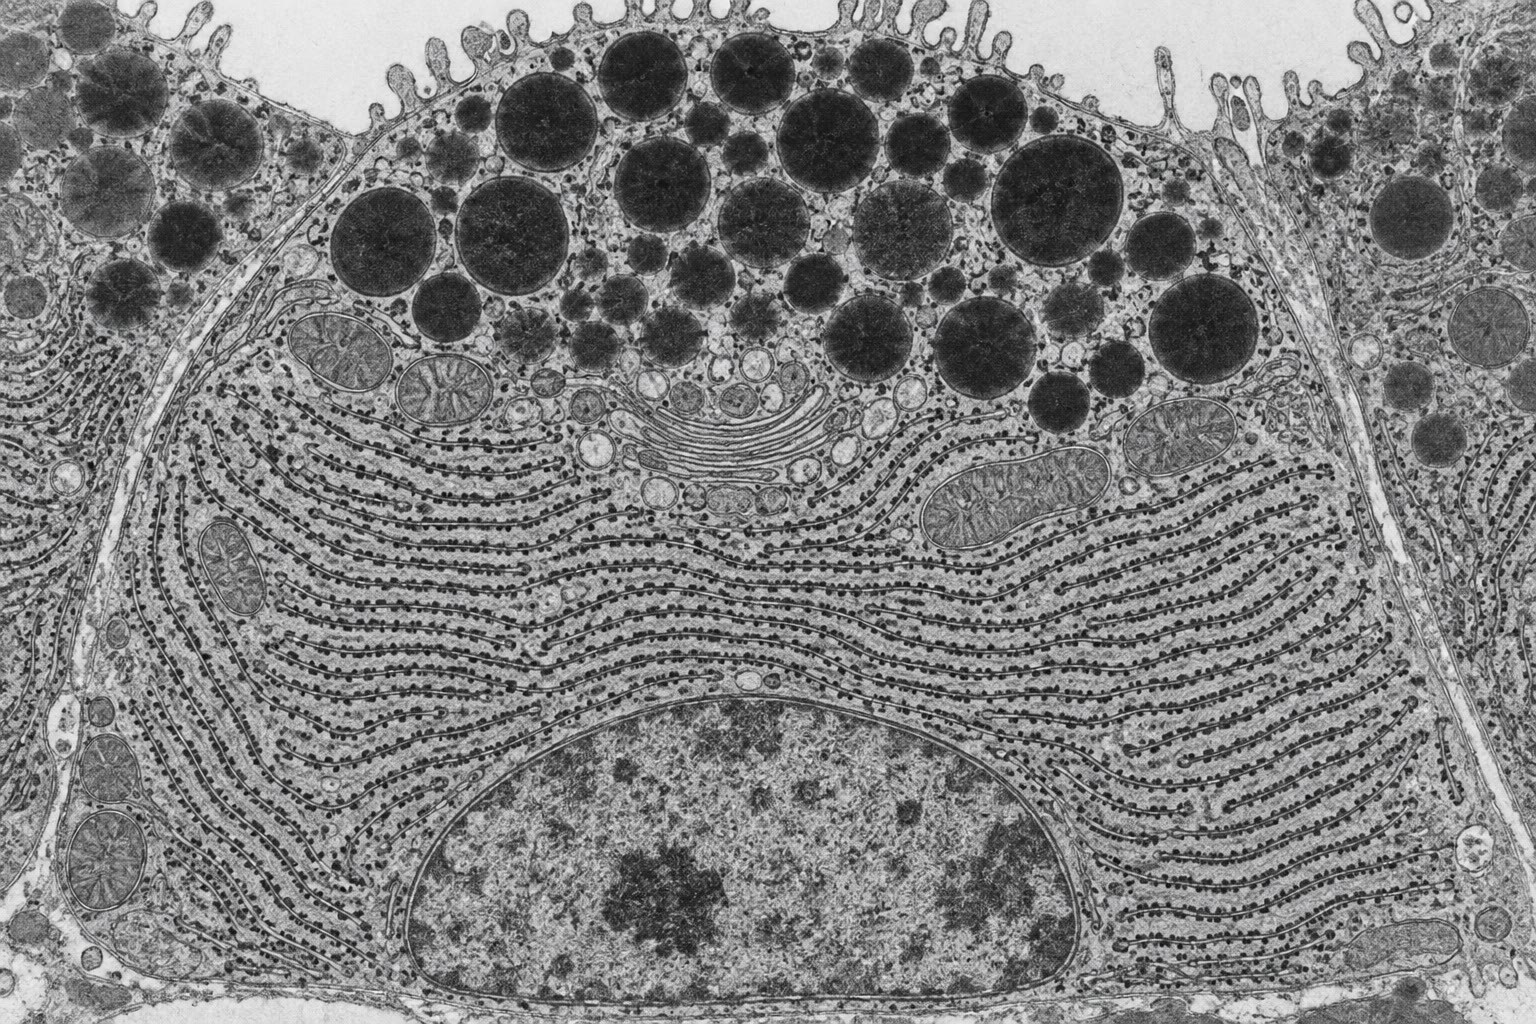
\includegraphics[width=0.56\linewidth]{images/book5/ai/b5-08-pancreas-acinar.jpg}

{\small इलेक्ट्रॉन सूक्ष्मदर्शी में अग्न्याशय की कोई कूपिका-कोशिका:
राइबोसोमों से जड़ी, ढेर लगी खुरदरी अंतर्द्रव्यी जालिका आधार भरती है,
गॉल्जी केंद्रक के ऊपर पड़ा है, और पाचक एंज़ाइम की सघन स्रावी कणिकाएँ
शीर्षस्थ पृष्ठ के नीचे भरी हैं, किसी संकेत की प्रतीक्षा में।}
\end{omfigure}

\section{पुटिकाएँ: मुकुलन, लक्ष्यन, संलयन}

\begin{definition}[आवरण और पुटिका-मुकुलन]\label{def:b3:membrane-traffic:coats}
\index{आवरित पुटिका}\index{COPII}\index{COPI}\index{क्लैथ्रिन}\index{लघु GTPase}
किसी परिवहन पुटिका को प्रोटीनों का कोई \emph{आवरण} आकार देता है, जो
किसी झिल्ली के कोशिकाद्रव्यी फलक पर जुड़ता है, झिल्ली को
\qtyrange{60}{100}{nm} की किसी कली में मोड़ता है, झिल्ली के आर-पार जाते
ग्राहियों से भार बटोरता है, और पुटिका के चिटक जाने के बाद उतार दिया
जाता है। मुख्य मार्गों पर तीन आवरण काम करते हैं: जालिका से गॉल्जी की ओर
जाती पुटिकाओं के लिए \emph{COPII}, गॉल्जी से जालिका तक की और गॉल्जी
कुंडों के बीच की वापसी यातायात के लिए \emph{COPI}, और
\emph{क्लैथ्रिन} --- तीन टाँगों वाला ऐसा प्रोटीन जो षट्भुजों और
पंचभुजों के पिंजरे में बहुलकित होता है --- ट्रांस-गॉल्जी से \omterm{def:b3:membrane-traffic:endocytosis}{अंतःकायों}
की ओर जाती पुटिकाओं के लिए और जीवद्रव्य-कला पर अंतर्ग्रहण के लिए, जहाँ
संयोजक प्रोटीन पिंजरे को भीतर लिए जा रहे ग्राहियों से जोड़ देते हैं।
हर आवरण को कोई \emph{लघु GTPase} बुलाती है (COPII के लिए Sar1, COPI और
क्लैथ्रिन के लिए Arf1), जो अपने GTP रूप में झिल्ली में घुस जाती है और
मुकुलन के बाद GTP का जल-अपघटन करके आवरण गिरा देती है। वापसी-संकेत
कक्षों को अलग-अलग बनाए रखते हैं: KDEL ढोते जो जालिका-प्रोटीन निकल भागें
उन्हें गॉल्जी में कोई ग्राही बाँध लेता है और COPI पुटिकाओं में वापस ले
जाता है।
\end{definition}

\begin{omfigure}
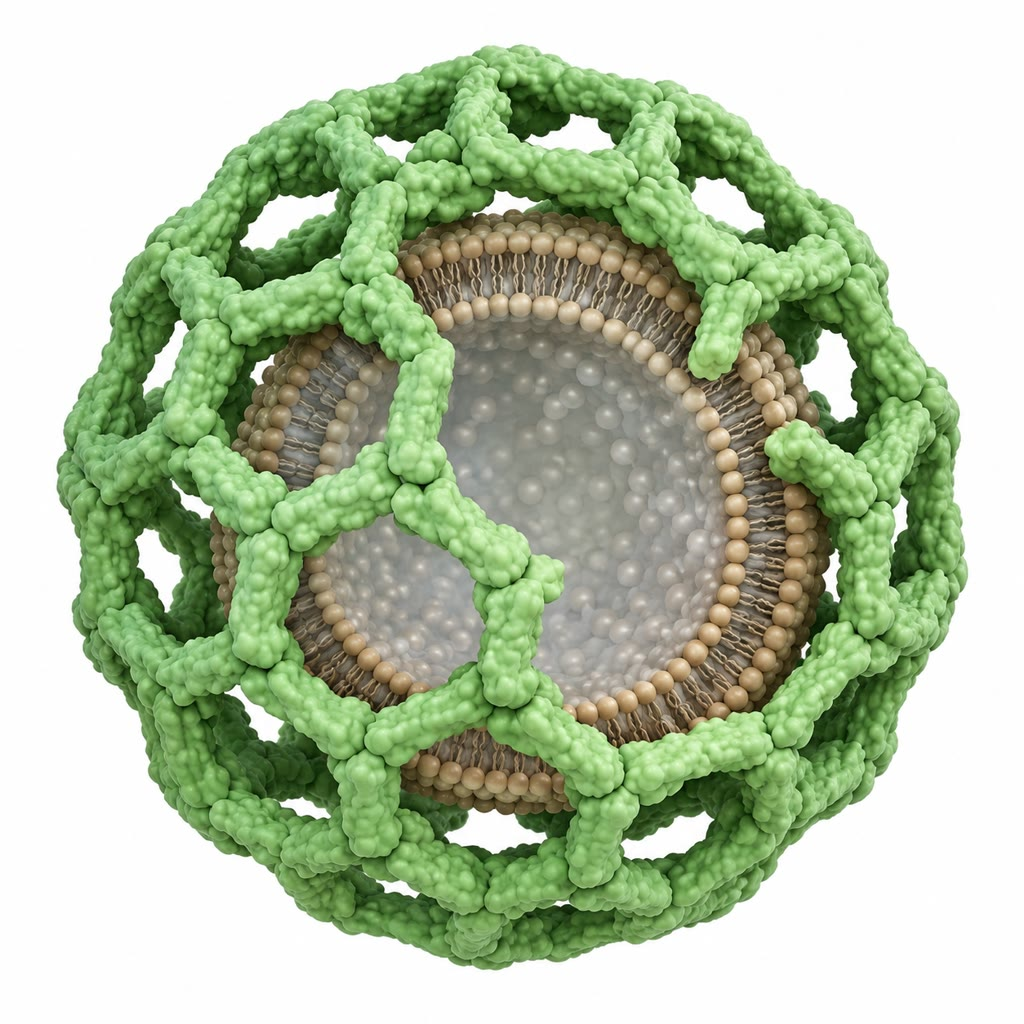
\includegraphics[width=0.36\linewidth]{images/book5/ai/b5-08-clathrin-cage.jpg}\hspace{0.04\linewidth}
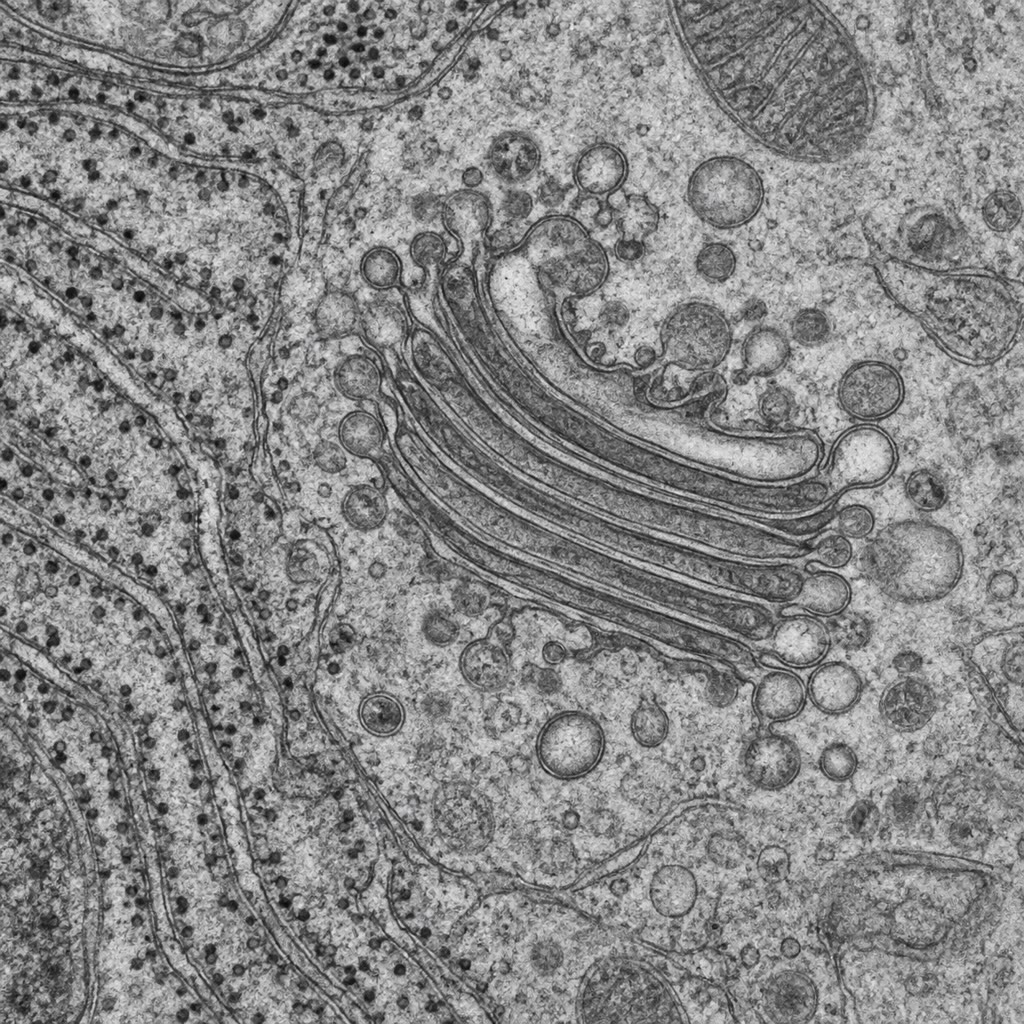
\includegraphics[width=0.36\linewidth]{images/book5/ai/b5-08-golgi-tem.jpg}

{\small बाएँ: कोई \omterm{def:b3:membrane-traffic:coats}{क्लैथ्रिन} पिंजरा, तीन-टाँग इकाइयों का वह बहुफलकी
जालक जो किसी अंतर्ग्राही पुटिका को आकार देता है (भीतर की झिल्ली दिखाने
के लिए काटकर)। दाएँ: इलेक्ट्रॉन सूक्ष्मदर्शी में कोई गॉल्जी ढेर, चपटे
कुंडों का ढेर जिनके किनारों से पुटिकाएँ मुकुलित हो रही हैं।}
\end{omfigure}

\begin{definition}[लक्ष्यन और संलयन]\label{def:b3:membrane-traffic:fusion}
\index{Rab GTPase}\index{SNARE}\index{झिल्ली संलयन}\index{सिनैप्टोटैगमिन}
कोई पुटिका अपना लक्ष्य पहचान की दो परतों से ढूँढ़ती है। \emph{Rab
GTPase} --- किसी मानव कोशिका में कोई साठ, हर एक किसी एक कक्ष की
झिल्लियों पर --- ऐसे लंबे रज्जु-प्रोटीन बुलाती हैं जो मेल खाता Rab ढोती
आती पुटिका को पकड़ लेते हैं। फिर \emph{SNARE} काम करते हैं: पुटिका पर
कोई v-SNARE और लक्ष्य पर t-SNARE, यानी अपनी झिल्लियों में जड़े कुंडलित
प्रोटीन, अपने दूरस्थ सिरों से झिल्लियों की ओर एक-दूसरे के चारों ओर
लिपटते हैं, और वे जो चार-कुंडली गट्ठर बनाते हैं उसकी ऊर्जा दोनों
द्विपरतों को तब तक पास खींचती है जब तक वे संलयित न हो जाएँ। हर SNARE
जोड़ी विशिष्ट है, पते की दूसरी जाँच। संलयन के बाद गट्ठर को ATPase NSF
फिर से काम में लेने के लिए अलग कर देती है। संलयन को किसी संकेत की
प्रतीक्षा करने को कहा जा सकता है: तंत्रिका-सिरे में SNARE को कॉम्प्लेक्सिन
आधा-लिपटा थामे रखता है जब तक \emph{सिनैप्टोटैगमिन}, किसी क्रिया-विभव के
आने पर घुसते कैल्शियम से बँधकर, एक मिलीसेकंड से भी कम में लिपटाई पूरी न
कर दे --- तंत्रिका-संचारक का वह मोचन जो वर्ष~2 के खंड में लिया गया है।
धनुस्तंभ और विषखाद्यता के तंत्रिकाविष ऐसे प्रोटिएज़ हैं जो SNARE काट
देते हैं।
\end{definition}

\begin{proof}[प्रमाण-सामग्री]
नोविक और शेकमन (1980) ने ताप-संवेदी खमीर उत्परिवर्ती अलग किए जो
\qty{37}{\celsius} पर स्राव बंद कर देते थे और उसी कक्ष में प्रोटीन जमा
कर लेते थे जहाँ उनका दोष रोक लगाता था --- जालिका, गॉल्जी, या पृष्ठ के
नीचे ढेर लगी पुटिकाएँ; $23$ \emph{sec} जीनों ने चरण परिभाषित किए और,
क्लोनित होने पर, वे आवरणों, GTPase और \omterm{def:b3:membrane-traffic:fusion}{SNARE} का कूटलेखन करते निकले।
रॉथमन ने गॉल्जी कुंडों के बीच परिवहन को परखनली में शुद्ध झिल्लियों,
कोशिकाद्रव्य और ATP के साथ फिर से खड़ा किया, और उसी से NSF तथा \omterm{def:b3:membrane-traffic:fusion}{SNARE}
शुद्ध किए; दोनों उपाय उन्हीं प्रोटीनों पर आकर मिले, और खमीर तथा
स्तनधारी मशीनें एक ही निकलीं।
\end{proof}

\begin{omfigure}
\begin{tikzpicture}[every node/.style={font=\scriptsize}, >=stealth]
  % three stages left to right
  \foreach \x/\gap/\lab in {0/1.2/{1. Rab से बँधी}, 4.4/0.55/{2. SNARE लिपटते हैं}, 8.8/0.0/{3. संलयन, भार मुक्त}} {
    % target membrane
    \draw[very thick, omDef] (\x,0) -- (\x+3.4,0); \draw[very thick, omDef] (\x,-0.3) -- (\x+3.4,-0.3);
    \node[below, align=center] at (\x+1.7,-0.45) {\lab};
  }
  % stage 1 vesicle
  \draw[very thick, omProp] (1.7,1.2+0.8) circle (0.8); \draw[very thick, omProp] (1.7,1.2+0.8) circle (0.6);
  \draw[omThm, thick] (1.4,1.25) -- (1.4,0.35); \draw[omThm, thick] (2.0,1.25) -- (2.0,0.35);
  \draw[omMeth!70!black, thick] (1.7,1.2) -- (1.7,0.6); \draw[omMeth!70!black, thick] (1.7,0.6) -- (1.7,0.0);
  \draw[thick, fill=omExo!40] (0.7,0.9) ellipse (0.25 and 0.2); \node[left] at (0.45,0.9) {Rab};
  \draw[thick, omExo!70!black] (0.95,0.9) .. controls (1.1,0.5) .. (1.2,0.05); \node[left, font=\tiny] at (0.9,0.4) {रज्जु};
  \node[right, font=\tiny] at (2.05,0.8) {SNARE};
  % stage 2 vesicle closer, helices twisted
  \draw[very thick, omProp] (6.1,0.55+0.8) circle (0.8); \draw[very thick, omProp] (6.1,0.55+0.8) circle (0.6);
  \draw[omThm, very thick] (5.85,0.6) .. controls (6.2,0.5) and (5.9,0.3) .. (6.1,0.05);
  \draw[omMeth!70!black, very thick] (6.35,0.6) .. controls (6.0,0.5) and (6.3,0.3) .. (6.1,0.05);
  \node[right, font=\tiny, align=left] at (6.6,0.35) {चार-कुंडली गट्ठर\\झिल्लियों को पास\\खींचता है};
  % stage 3 fused omega shape
  \draw[very thick, omProp] (9.7,0) .. controls (9.7,1.5) and (11.3,1.5) .. (11.3,0);
  \draw[very thick, omProp] (9.9,-0.3) .. controls (9.9,1.1) and (11.1,1.1) .. (11.1,-0.3);
  \foreach \p in {(10.5,-0.9),(10.2,-1.1),(10.8,-1.15)} \fill[omExo] \p circle (0.06);
  \draw[->, omExo, thick] (10.5,0.5) -- (10.5,-0.6);
  \node[right, font=\tiny, align=left] at (11.4,0.8) {बाद में NSF\\SNARE को\\खोल देती है};
\end{tikzpicture}

{\small तीन चरणों में संलयन। पुटिका पर कोई Rab और लक्ष्य पर कोई रज्जु
दोनों झिल्लियों को पहुँच के भीतर ले आते हैं; पुटिका और लक्ष्य के
\omterm{def:b3:membrane-traffic:fusion}{SNARE} (लाल और हरे) किसी चार-कुंडली गट्ठर में लिपट जाते हैं जो
द्विपरतों को घसीटकर पास ले आता है; वे संलयित होते हैं और भार लक्ष्य
कक्ष में चला जाता है।}
\end{omfigure}

\begin{proposition}[गॉल्जी]\label{prop:b3:membrane-traffic:golgi}
\index{गॉल्जी उपकरण}\index{कुंड-परिपक्वन}\index{मैनोज़-6-फ़ॉस्फ़ेट}
गॉल्जी चार से आठ चपटे कुंडों का ढेर है, जिसका सिस फलक जालिका की ओर और
ट्रांस फलक जीवद्रव्य-कला की ओर है, और हर कुंड में एंज़ाइमों का अलग
समुच्चय रहता है जो गुज़रते ग्लाइकोप्रोटीनों की शर्कराएँ छाँटता और फिर
बनाता है तथा O-सहलग्न शर्कराएँ, सल्फ़ेट और फ़ॉस्फ़ेट जोड़ता है। भार
मुख्यतः \emph{\omterm{prop:b3:membrane-traffic:golgi}{कुंड-परिपक्वन}} से आगे बढ़ता है: सिस फलक पर आती पुटिकाओं
से कोई नया कुंड बनता है, अपने से पहले वालों की तरह ढेर से होकर चलता है,
और परिपक्व होता जाता है क्योंकि \omterm{def:b3:membrane-traffic:coats}{COPI} पुटिकाएँ हर कुंड के एंज़ाइम पीछे
अपने से छोटे कुंड तक ले जाती हैं; ट्रांस फलक पर वह अपने गंतव्यों को
जाती पुटिकाओं में टूट जाता है। वहीं छँटाई तय होती है: लयनकायी
जल-अपघटनी, जिन्हें सिस गॉल्जी में \emph{मैनोज़-6-फ़ॉस्फ़ेट} से अंकित
किया जाता है, अपने ग्राही से बँधकर \omterm{def:b3:membrane-traffic:endocytosis}{अंतःकाय} के लिए \omterm{def:b3:membrane-traffic:coats}{क्लैथ्रिन} पुटिकाओं
में भर दिए जाते हैं; नियमित स्रावी प्रोटीन हल्के अम्लीय pH पर पुंजित
होकर संघनक कणिकाएँ बना लेते हैं; बाकी सब पृष्ठ के लिए संघटक धारा में
निकल जाता है। I-कोशिका रोग में फ़ॉस्फ़ोरिलन करने वाला एंज़ाइम नहीं होता,
जल-अपघटनी पहुँचाए जाने के बजाय स्रावित हो जाते हैं, और \omterm{def:b3:membrane-traffic:endocytosis}{लयनकाय} अपचित
सामग्री से भर जाते हैं।
\end{proposition}

\begin{omfigure}
\begin{tikzpicture}[every node/.style={font=\scriptsize}, >=stealth]
  % plasma membrane top
  \draw[very thick, omDef] (0,4.2) -- (12,4.2); \node[above] at (6,4.25) {जीवद्रव्य-कला \quad (ऊपर बाहर)};
  % ER
  \draw[thick, fill=omDef!12] (0.3,0.0) rectangle (4.0,0.9); \node at (2.15,0.45) {अंतर्द्रव्यी जालिका};
  % Golgi stack
  \foreach \y in {1.5,1.85,2.2,2.55} \draw[thick, fill=omProp!25] (4.8,\y) ellipse (1.4 and 0.13);
  \node[right] at (6.3,1.5) {सिस}; \node[left] at (3.35,2.55) {ट्रांस};
  \node[right] at (6.3,2.05) {गॉल्जी ढेर};
  % ER -> Golgi (COPII)
  \draw[->, thick, omMeth!70!black] (3.9,0.95) -- (4.5,1.4); \node[right, omMeth!70!black, font=\tiny] at (4.35,1.02) {COPII};
  % Golgi -> ER (COPI)
  \draw[->, thick, omThm] (3.6,1.42) -- (2.9,0.95); \node[left, omThm, font=\tiny] at (2.95,1.3) {COPI, KDEL वापसी};
  % trans Golgi -> PM constitutive
  \draw[->, thick, omMeth!70!black] (5.6,2.7) -- (7.6,4.1); \node[left, font=\tiny, align=right] at (6.4,3.6) {संघटक\\स्राव};
  % trans -> secretory granule -> PM regulated
  \draw[->, thick, omMeth!70!black] (4.6,2.7) -- (4.0,3.3); \draw[thick, fill=omExo!50] (3.8,3.5) circle (0.22); \draw[->, thick, omMeth!70!black] (3.8,3.75) -- (3.8,4.1);
  \node[left, font=\tiny, align=right] at (3.55,3.5) {स्रावी कणिका:\\नियमित, किसी संकेत पर};
  % trans -> endosome/lysosome (clathrin, M6P)
  \draw[->, thick, omProp!80!black] (6.0,2.62) -- (8.25,2.62); \node[above, font=\tiny] at (7.1,2.67) {क्लैथ्रिन, M6P ग्राही};
  \draw[thick, fill=omProp!20] (8.8,2.7) circle (0.5); \node at (8.8,2.7) {\tiny अंतःकाय};
  \draw[->, thick, omProp!80!black] (9.25,2.4) -- (10.2,1.95); \draw[thick, fill=omThm!25] (10.7,1.6) circle (0.5); \node at (10.7,1.6) {\tiny लयनकाय};
  % endocytosis from PM to endosome
  \draw[->, thick, omDef] (9.6,4.15) -- (9.1,3.2); \node[right, font=\tiny, align=left] at (9.5,3.7) {अंतर्ग्रहण\\(क्लैथ्रिन गड्ढे)};
  % recycling endosome -> PM
  \draw[->, thick, omDef] (8.5,3.2) -- (8.0,4.15); \node[left, font=\tiny] at (8.3,3.3) {पुनर्चक्रण};
  % lysosome inputs autophagy
  \draw[->, thick, gray] (11.9,0.6) -- (11.1,1.3); \node[below, font=\tiny, align=center] at (11.9,0.55) {स्वभक्षी-काय\\(कोशिकाद्रव्य, कोशिकांग)};
\end{tikzpicture}

{\small झिल्ली यातायात का मानचित्र। बाहर की ओर (हरा): \omterm{def:b3:membrane-traffic:coats}{COPII} पुटिकाओं
में जालिका से गॉल्जी, गॉल्जी से पृष्ठ तक या तो संघटक रूप से या ऐसी
कणिकाओं से जो किसी संकेत की प्रतीक्षा करती हैं। पीछे की ओर (लाल): \omterm{def:b3:membrane-traffic:coats}{COPI}
पुटिकाएँ भागे हुए जालिका-प्रोटीन लौटाती हैं। नीचे की ओर (नारंगी):
मैनोज़-6-फ़ॉस्फ़ेट से अंकित लयनकायी एंज़ाइम \omterm{def:b3:membrane-traffic:endocytosis}{अंतःकाय} और \omterm{def:b3:membrane-traffic:endocytosis}{लयनकाय} तक जाते
हैं। भीतर की ओर (नीला): पृष्ठ से अंतर्ग्रहण, जिसमें अधिकांश ग्राही
पुनर्चक्रित होते हैं।}
\end{omfigure}

\section{अंतर्ग्रहण और लयनकाय}

\begin{definition}[अंतर्ग्रहण]\label{def:b3:membrane-traffic:endocytosis}
\index{ग्राही-मध्यस्थ अंतर्ग्रहण}\index{अंतःकाय}\index{लयनकाय}\index{स्वभक्षण}
\emph{ग्राही-मध्यस्थ अंतर्ग्रहण} पृष्ठ-ग्राहियों से बँधे किसी लिगंड को
क्लैथ्रिन-आवरित गड्ढों में सांद्र कर देता है, जो लगभग \qty{100}{nm} की
पुटिकाओं के रूप में चिटक जाते हैं (GTPase डायनामिन गरदन कस देती है)
--- किसी तंतुकोरक में प्रति मिनट एक हज़ार, जो पूरी पृष्ठ-झिल्ली एक घंटे
में बदल देते हैं। पुटिकाएँ \emph{अगेते
अंतःकायों} में संलयित होती हैं, जिनकी अवकाशिका किसी प्रोटॉन पंप से
pH~6 तक अम्लीय की जाती है; अधिकांश लिगंड वहीं अपने ग्राही छोड़ देते
हैं, \omterm{prop:b3:membrane-traffic:uptake}{ग्राही पुनर्चक्रण} पुटिकाओं में पृष्ठ पर लौट आते हैं, और लिगंड आगे
चलता जाता है क्योंकि अंतःकाय परिपक्व होकर पछेता अंतःकाय (pH~5.5) बनता
है और किसी \emph{लयनकाय} से संलयित होता है: वह कक्ष जो pH~4.5--5 पर
कोई साठ जल-अपघटनी --- प्रोटिएज़, न्यूक्लिएज़, लाइपेज़, ग्लाइकोसिडेज़
--- रखता है, जो केवल उसी pH पर सक्रिय रहती हैं, ताकि उदासीन
कोशिकाद्रव्य में कोई रिसाव थोड़ी ही हानि करे। लयनकाय कोशिका की अपनी वह
सामग्री भी पचाता है जो \emph{स्वभक्षण} से पहुँचती है: कोई दोहरी झिल्ली
कोशिकाद्रव्य के किसी भाग या किसी घिसे कोशिकांग के चारों ओर बढ़ती है,
किसी स्वभक्षी-काय में बंद हो जाती है, और लयनकाय से संलयित होती है;
उत्पाद कोशिकाद्रव्य में लौटा दिए जाते हैं। स्वभक्षण भुखमरी से प्रेरित
होता है (वह ऊर्जा के लिए कोशिका का अपना ही पदार्थ पुनर्चक्रित करता है)
और पुंज तथा क्षतिग्रस्त सूत्रकणिकाएँ साफ़ करता है; उसकी विफलता
तंत्रिका-अपह्रास में फँसाई गई है।
\end{definition}

\begin{proof}[प्रमाण-सामग्री]
ब्राउन और गोल्डस्टाइन (1970 के दशक) ने अल्प-घनत्व लिपोप्रोटीन (LDL) का,
यानी रक्त में कोलेस्टेरॉल ढोते कण का, संवर्धित तंतुकोरकों में पीछा
किया। LDL प्रति कोशिका कोई \num{20000} पृष्ठ-स्थलों से संतृप्य रूप से
बँधा, मिनटों में आवरित गड्ढों में भीतर लिया गया, और उसका
कोलेस्टेरॉल \omterm{def:b3:membrane-traffic:endocytosis}{लयनकायों} में मुक्त होकर कोशिका का अपना
कोलेस्टेरॉल-संश्लेषण बंद कर बैठा। कुलगत अतिकोलेस्टेरॉलरक्तता के
रोगियों के तंतुकोरकों ने या तो कोई LDL नहीं बाँधा (ग्राही अनुपस्थित) या
बाँधा पर भीतर नहीं लिया (ग्राही की कोशिकाद्रव्यी पुच्छ में ऐसा
उत्परिवर्तन जो \omterm{def:b3:membrane-traffic:coats}{क्लैथ्रिन} संयोजकों द्वारा उसे पकड़े जाने से रोकता है):
रोग अंतर्ग्रहण का दोष था, ग्राही की पुच्छ में आंतरिकीकरण-संकेत था, और
पुनर्चक्रित होता ग्राही --- हर एक सैकड़ों चक्कर लगाता --- ग्रहण की
सामान्य क्रियाविधि के रूप में स्थापित हो गया।
\end{proof}

\begin{proposition}[पुनर्चक्रित ग्राहियों से ग्रहण]\label{prop:b3:membrane-traffic:uptake}
\index{ग्राही पुनर्चक्रण}
मान लीजिए किसी कोशिका में कुल $R$ ग्राही हैं, जिनमें से $S$ पृष्ठ पर
हैं और $R - S$ भीतर लौटने के रास्ते पर। कोई पृष्ठ-ग्राही प्रायिकता
$\theta = [L]/(K_{d} + [L])$ से अधिकृत रहता है, कोई अधिकृत ग्राही दर
$k_{i}$ से भीतर लिया जाता है, और भीतर लिया गया कोई ग्राही दर
$k_{r}$ से लौटता है। स्थायी अवस्था पर कोशिका में लिगंड का अभिवाह है
\[
J = \frac{R\,k_{i}k_{r}\,\theta}{k_{r} + k_{i}\theta},
\]
जो लिगंड सांद्रता बढ़ने पर $J_{\max} =
R\,k_{i}k_{r}/(k_{i} + k_{r})$ पर संतृप्त हो जाता है: किसी कोशिका का
ग्रहण केवल उसके ग्राहियों से नहीं, बल्कि इससे भी सीमित है कि वह उन्हें
कितनी तेज़ी से वापस ला सकती है।
\end{proposition}
\begin{proof}
पृष्ठ-ग्राही दर $k_{i}\theta S$ से खोते हैं और दर
$k_{r}(R - S)$ से फिर मिलते हैं; स्थायी अवस्था पर ये बराबर होते हैं,
इसलिए $S = R\,k_{r}/(k_{r}
+ k_{i}\theta)$। हर आंतरिकीकरण एक लिगंड ले जाता है, इसलिए $J =
k_{i}\theta S$, जिससे सूत्र मिलता है। $\theta \to 1$ पर अभिवाह
$R\,k_{i}k_{r}/(k_{r} + k_{i})$ की ओर जाता है --- ग्राही उतनी ही तेज़ी
से चक्कर लगाते हैं जितनी दोनों दरें देती हैं, और किसी भी क्षण उनका
$k_{r}/(k_{i} + k_{r})$ अंश पृष्ठ पर रहता है।
\end{proof}

\begin{example}[कण-दर-कण LDL]\label{ex:b3:membrane-traffic:ldl}
$R = \num{20000}$ LDL ग्राहियों, \qty{5}{min} के आंतरिकीकरण-काल
($k_{i} = \qty{0.2}{min^{-1}}$) और \qty{10}{min} के वापसी-काल
($k_{r} = \qty{0.1}{min^{-1}}$) वाला कोई तंतुकोरक, संतृप्त करने वाले
LDL पर, $J_{\max} = \num{20000}\times 0.2\times 0.1/0.3 \approx 1300$
कण प्रति मिनट ग्रहण करता है, और किसी भी क्षण उसके एक-तिहाई ग्राही पृष्ठ
पर रहते हैं; हर कण कोई \num{1500} कोलेस्टेरॉल अणु लाता है, यानी प्रति
मिनट बीस लाख, जो लगभग एक-दसवाँ वर्ग माइक्रोमीटर झिल्ली बनाने के लिए
पर्याप्त है। कुलगत अतिकोलेस्टेरॉलरक्तता का कोई विषमयुग्मजी, जिसके पास
आधे ग्राही हैं, आधा ही ग्रहण करता है; रक्त-कोलेस्टेरॉल दोगुना हो जाता
है, और हृद्रोग बीस वर्ष पहले आ जाता है। स्टैटिन यकृत-कोशिका को उसके
अपने कोलेस्टेरॉल से वंचित करके $R$ बढ़ा देते हैं।
\end{example}

\begin{omfigure}
\begin{tikzpicture}
\begin{axis}[
  width=0.7\linewidth, height=5.4cm,
  axis x line=bottom, axis y line=left,
  xmin=0, xmax=10, ymin=0, ymax=1500,
  xlabel={LDL सांद्रता, $[L]/K_{d}$}, ylabel={कण प्रति मिनट},
  xlabel style={font=\small, at={(axis description cs:0.5,-0.12)}, anchor=north},
  ylabel style={font=\small},
  tick label style={font=\small}, xtick={0,2,4,6,8,10}, ytick={0,500,1000,1333}, yticklabels={0,500,1000,$J_{\max}$},
  clip=false,
]
\addplot[very thick, omDef, domain=0:10, samples=60] {20000*0.2*0.1*(x/(1+x))/(0.1+0.2*(x/(1+x)))};
\addplot[very thick, omThm, domain=0:10, samples=60] {10000*0.2*0.1*(x/(1+x))/(0.1+0.2*(x/(1+x)))};
\addplot[dashed, gray, domain=0:10, samples=2] {1333};
\node[font=\scriptsize, omDef, anchor=north west] at (axis cs:4,900) {$R = \num{20000}$};
\node[font=\scriptsize, omThm, anchor=north west] at (axis cs:4,560) {$R = \num{10000}$ (विषमयुग्मजी)};
\end{axis}
\end{tikzpicture}

{\small $k_{i} = \qty{0.2}{min^{-1}}$ और $k_{r} =
\qty{0.1}{min^{-1}}$ के साथ प्रतिज्ञप्ति के सूत्र से पुनर्चक्रित
ग्राहियों द्वारा LDL का ग्रहण: लिगंड के साथ संतृप्त होता, और आधे ग्राही
न होने पर आधा।}
\end{omfigure}

\begin{remark}[एक झिल्ली, अनेक कक्ष]\label{rem:b3:membrane-traffic:one-membrane}
स्रावी और अंतर्ग्राही तंत्र की हर झिल्ली, सांस्थिति की दृष्टि से,
एक ही झिल्ली है: जालिका की अवकाशिका पुटिकाओं के ज़रिए कोशिका के बाहर से
सतत जुड़ी है, और जालिका में बना कोई लिपिड या प्रोटीन बिना किसी द्विपरत
को पार किए पृष्ठ तक पहुँच सकता है। कक्षों को अलग दीवारें नहीं, यातायात
रखता है --- चुनिंदा बाहर भरना, चुनिंदा वापस लाना, और हर संलयन पर पहचान
के अणुओं की कोई विशिष्ट जोड़ी। कक्ष प्रवाहों की स्थायी अवस्थाएँ हैं,
किसी नदी के कुंडों की तरह, और जो कोशिका यातायात बंद कर दे वह घंटों में
अपना भूगोल खो देती है।
\end{remark}

\section{अभ्यास}

\begin{exercise}[$\star$]\label{exo:b3:membrane-traffic:1}
हर एक के लिए संकेत और गंतव्य दीजिए: अमीनो सिरे पर बीस जलविरोधी अवशेषों
का कोई खंड; PKKKRKV; अमीनो-सिरे की कोई उभयरागी कुंडली; कार्बोक्सी सिरे
पर KDEL; शर्कराओं पर कोई
मैनोज़-6-फ़ॉस्फ़ेट।
\end{exercise}

\begin{exercise}[$\star$]\label{exo:b3:membrane-traffic:2}
ब्लोबेल--डॉबरश्टाइन प्रयोग के तीन मुख्य प्रेक्षणों का वर्णन कीजिए और
बताइए कि हर एक ने क्या दिखाया।
\end{exercise}

\begin{exercise}[$\star$]\label{exo:b3:membrane-traffic:3}
इनके लिए \omterm{def:b3:membrane-traffic:coats}{आवरण} और परिवहन की दिशा बताइए: जालिका से गॉल्जी; गॉल्जी से
जालिका; ट्रांस-गॉल्जी से \omterm{def:b3:membrane-traffic:endocytosis}{अंतःकाय}; जीवद्रव्य-कला से \omterm{def:b3:membrane-traffic:endocytosis}{अंतःकाय}।
\end{exercise}

\begin{exercise}[$\star$]\label{exo:b3:membrane-traffic:4}
किसी जीवद्रव्य-कला प्रोटीन की शर्कराएँ सदा कोशिका के बाहर की ओर क्यों
होती हैं?
\end{exercise}

\begin{exercise}[$\star\star$]\label{exo:b3:membrane-traffic:5}
\cref{thm:b3:membrane-traffic:pulse-chase} के प्रतिरूप में $k_{1}
= \qty{0.2}{min^{-1}}$ और $k_{2} = \qty{0.05}{min^{-1}}$ के साथ ढूँढ़िए
कि गॉल्जी का चिह्न कब शिखर छूता है और शिखर पर वहाँ कितना है; फिर
\qty{60}{min} पर कणिकाओं में अंश।
\end{exercise}

\begin{exercise}[$\star\star$]\label{exo:b3:membrane-traffic:6}
किसी झिल्ली प्रोटीन में स्थिति 30, 90, 150 और 210 पर $22$ अवशेषों के
जलविरोधी खंड हैं और अमीनो सिरे पर कोई \omterm{def:b3:membrane-traffic:signals}{संकेत पेप्टाइड}।
उसकी सांस्थिति खींचिए या उसका वर्णन कीजिए: कितनी कुंडलियाँ, और उनके
बीच का हर खंड किस ओर है? उसका ग्लाइकोसिलन कहाँ हो सकता है?
\end{exercise}

\begin{exercise}[$\star\star$]\label{exo:b3:membrane-traffic:7}
$R = \num{30000}$,
$k_{i} = \qty{0.25}{min^{-1}}$, $k_{r} = \qty{0.05}{min^{-1}}$ के साथ
\cref{prop:b3:membrane-traffic:uptake} का उपयोग करते हुए
$J_{\max}$ और संतृप्ति पर पृष्ठ के ग्राहियों का अंश निकालिए।
कौन-सा एक बदलाव ग्रहण दोगुना कर देगा?
\end{exercise}

\begin{exercise}[$\star\star$]\label{exo:b3:membrane-traffic:8}
(क) मैनोज़-6-फ़ॉस्फ़ेट ग्राही से वंचित कोशिका, (ख) वह अंकक जोड़ने वाली
फ़ॉस्फ़ोट्रांसफ़रेज़ से वंचित कोशिका, (ग) अंतःकायी pH उदासीन करने वाली
किसी औषध से उपचारित कोशिका --- इनमें लयनकायी जल-अपघटनियों की नियति और
लक्षण-प्ररूप का पूर्वानुमान कीजिए।
\end{exercise}

\begin{exercise}[$\star\star$]\label{exo:b3:membrane-traffic:9}
LDL ग्राही का JD उत्परिवर्तन कोशिकाद्रव्यी पुच्छ के किसी टायरोसीन को
बदल देता है। जो कोशिकाएँ LDL सामान्य रूप से बाँधती हैं वे उसे भीतर नहीं
ले पातीं। क्रियाविधि समझाइए, और पूर्वानुमान कीजिए कि कोशिका-पृष्ठ पर
आवरित गड्ढों के सापेक्ष ग्राही कहाँ मिलेंगे।
\end{exercise}

\begin{exercise}[$\star\star\star$]\label{exo:b3:membrane-traffic:10}
स्फुरण--अनुधावन प्रतिरूप को $k_{1} = k_{2} = k$ की स्थिति के लिए हल
कीजिए (वहाँ प्रमेय का सूत्र विचित्र हो जाता है): दिखाइए कि $B(t) = kt\,e^{-kt}$
है और शिखर ढूँढ़िए। फिर समझाइए कि केवल कणिका-अंश
$C(t)$ मापने से दोनों दरें अलग-अलग क्यों तय नहीं की जा सकतीं।
\end{exercise}

\begin{exercise}[$\star\star\star$]\label{exo:b3:membrane-traffic:11}
कोई तंतुकोरक प्रति मिनट \qty{100}{nm} व्यास की \num{1000} \omterm{def:b3:membrane-traffic:coats}{क्लैथ्रिन}
पुटिकाएँ भीतर लेता है और उसका पृष्ठ \qty{3000}{\micro m^2} है। पूरे
पृष्ठ के बराबर भीतर लेने में कितना समय लगेगा? कोशिका सिकुड़ती क्यों
नहीं, और इस संतुलन से बहिर्ग्रहण की दर और प्रति घंटा भीतर लिए गए द्रव
के आयतन के बारे में क्या निकलता है?
\end{exercise}

\begin{exercise}[$\star\star\star$]\label{exo:b3:membrane-traffic:12}
बोटुलिनम विष चालक तंत्रिका-सिरों में कोई \omterm{def:b3:membrane-traffic:fusion}{SNARE} काटता है; धनुस्तंभ विष
मेरुरज्जु के निरोधी अंतर्न्यूरॉनों में वही \omterm{def:b3:membrane-traffic:fusion}{SNARE} काटता है। समझाइए कि
पहला शिथिल और दूसरा स्पास्टिक पक्षाघात क्यों करता है, और संलयन रोकने
वाला कोई विष चिकित्सा में सूक्ष्म मात्राओं में क्यों उपयोगी है।
\end{exercise}

\section{समस्या: अग्न्याशय की किसी कोशिका का एक दिन}

\begin{problem}[{सप्तांत समस्या --- किसी स्रावी कोशिका का उत्पादन अणुओं,
पुटिकाओं और वर्ग माइक्रोमीटरों में गिना गया, उसके स्फुरण--अनुधावन वक्र
हल किए गए, यकृत की किसी कोशिका का कोलेस्टेरॉल-ग्रहण पुनर्चक्रित
ग्राहियों से निकाला गया, और कोई लयनकाय प्रोटॉन-दर-प्रोटॉन अम्लीय किया
गया, जिसका अंत गॉल्जी शिखर के समय, प्रति मिनट मुकुलित पुटिकाओं और प्रति
घंटा ग्रहण किए गए LDL कणों पर होता है}]
\label{pb:b3:membrane-traffic:1}
आँकड़े: कोई कूपिका-कोशिका प्रति मिनट $10^{7}$ एंज़ाइम अणु बनाती है, हर एक
\qty{25}{kDa} का, \qty{4}{nm} चौड़ा। परिवहन पुटिकाएँ
\qty{70}{nm} व्यास के गोले हैं; कोई कणिका \qty{1}{\micro m} का गोला है।
प्रति लिपिड अणु झिल्ली-क्षेत्रफल \qty{0.7}{nm^2}, दो परतें। कोशिका की
जालिका का क्षेत्रफल \qty{6000}{\micro m^2} है। स्फुरण--अनुधावन:
$k_{1} = \qty{0.1}{min^{-1}}$, $k_{2} = \qty{0.05}{min^{-1}}$। यकृत की
कोई कोशिका: $R = \num{50000}$ LDL ग्राही, $k_{i} = \qty{0.2}{min^{-1}}$,
$k_{r} = \qty{0.1}{min^{-1}}$, $K_{d} = \qty{2}{nmol/L}$, प्लाज़्मा LDL
कण-सांद्रता \qty{2}{nmol/L}; प्रति कण \num{1500} कोलेस्टेरॉल अणु।
कोई \omterm{def:b3:membrane-traffic:endocytosis}{लयनकाय}: \qty{0.5}{\micro m} का गोला, pH $7.2$ से $4.7$ तक,
और बफ़री क्षमता ऐसी कि हर एक मुक्त बचे प्रोटॉन के लिए $50$ प्रोटॉन पंप
करने पड़ते हैं; कोई प्रोटॉन पंप प्रति सेकंड $200$ प्रोटॉन चलाता है।

\medskip
\noindent\textbf{भाग I --- उत्पादन।}
\begin{enumerate}
  \item कोशिका प्रति मिनट और प्रति दिन कितने द्रव्यमान का एंज़ाइम
        बनाती है? कोशिका की अपनी प्रोटीन-मात्रा, लगभग
        \qty{300}{pg}, से तुलना कीजिए।
  \item यदि एंज़ाइम अणु किसी पुटिका के आयतन का \qty{30}{\%} भरें
        (\qty{4}{nm} का गोला) तो एक पुटिका में कितने अटते हैं? प्रति
        मिनट कितनी पुटिकाएँ जालिका से निकलती हैं?
  \item वे पुटिकाएँ प्रति मिनट कितना झिल्ली-क्षेत्रफल ढोती हैं, और यदि
        कुछ भी वापस न आए तो वे पूरी जालिका कितने समय में खपा देंगी?
  \item वह प्रति मिनट कितने लिपिड अणु हुए? अपनी जालिका बचाए रखने के
        लिए कोशिका को क्या करना पड़ता है?
  \item उसी जमाव पर किसी कणिका में कितने एंज़ाइम अणु अटते हैं, और
        कोशिका प्रति घंटा कितनी कणिकाएँ भरती है?
  \item कोई भोजन दस मिनट में $300$ कणिकाएँ शीर्षस्थ झिल्ली से संलयन
        द्वारा खाली कर देता है और उनकी झिल्ली
        \qty{50}{\micro m^2} के किसी पृष्ठ में जोड़ देता है। शीर्षस्थ
        पृष्ठ किस गुणक से बढ़ता है, और उसके बाद क्या होना चाहिए?
\end{enumerate}

\medskip
\noindent\textbf{भाग II --- समय-निर्धारण।}
\begin{enumerate}[resume]
  \item दी हुई दरों के साथ गॉल्जी का चिह्न कब शिखर छूता है, और वहाँ
        कितना अंश है?
  \item \qty{30}{min} पर किसी स्फुरण का कितना अंश जालिका, गॉल्जी और
        कणिकाओं में है?
  \item दोनों कक्षों में माध्य निवास-काल? संश्लेषण से कणिका तक माध्य
        कुल समय क्या है?
  \item कोई औषध गॉल्जी से निकास को $k_{2} = \qty{0.01}{min^{-1}}$ तक
        धीमा कर देती है। नया शिखर-समय और शिखर-अंश; सूक्ष्मदर्शी में
        गॉल्जी कैसा दिखता है?
  \item समझाइए कि गॉल्जी का शिखर-अंश $k_{1}/k_{2}$ की किसी घात
        (घात बताइए) के रूप में क्यों है और इसलिए सदा $1$ से नीचे रहता है।
  \item यदि जालिका का चरण गॉल्जी के चरण से बहुत तेज़ होता, तो $B(t)$
        किसकी ओर जाता? व्याख्या कीजिए।
\end{enumerate}

\medskip
\noindent\textbf{भाग III --- कोलेस्टेरॉल।}
\begin{enumerate}[resume]
  \item प्लाज़्मा LDL सांद्रता पर $\theta$ निकालिए, और ग्रहण
        $J$ कणों में प्रति मिनट तथा प्रति घंटा।
  \item प्रति घंटा कितने कोलेस्टेरॉल अणु? कोशिका की झिल्लियों में
        $5\times 10^{9}$ कोलेस्टेरॉल अणु हैं; केवल LDL से उन सबको
        बदलने में कितना समय लगेगा?
  \item पृष्ठ के ग्राहियों का अंश, और हर ग्राही अपने \qty{20}{h}
        जीवन-काल में कितने चक्कर लगाता है, निकालिए।
  \item किसी विषमयुग्मजी के पास $R = \num{25000}$ है: $J$ फिर से
        निकालिए। प्लाज़्मा LDL तब तक बढ़ता है जब तक ग्रहण उत्पादन के
        बराबर न हो जाए: यदि $\theta$ संतृप्ति से काफ़ी नीचे हो तो किस
        गुणक से?
  \item कोई स्टैटिन विषमयुग्मजी की यकृत-कोशिकाओं में $R$ दोगुना कर
        देता है। उसी तर्क से प्लाज़्मा LDL का क्या होता है?
  \item समझाइए कि ग्राही-शून्य समयुग्मजी, जिसका प्लाज़्मा LDL सामान्य
        से पाँच गुना है, अकेले प्रश्न 16 के अंकगणित के सुझाव से भी
        बुरी हालत में क्यों है।
\end{enumerate}

\medskip
\noindent\textbf{भाग IV --- अम्ल।}
\begin{enumerate}[resume]
  \item \omterm{def:b3:membrane-traffic:endocytosis}{लयनकाय} का आयतन लीटरों में और pH $7.2$ तथा pH $4.7$ पर मुक्त
        प्रोटॉनों की संख्या निकालिए।
  \item बफ़री के साथ कुल कितने प्रोटॉन पंप करने पड़ेंगे? $50$ पंपों से
        उसमें कितना समय लगता है?
  \item पंप प्रोटॉनों को प्रवणता के विरुद्ध भीतर ले जाता है। कौन-सी
        वैद्युत समस्या उठती है, और वह कैसे हल होती है (किसी प्रति-आयन
        के बारे में सोचिए)?
  \item जल-अपघटनी केवल pH~5 पर ही सक्रिय क्यों बनाई जाती हैं, और यह
        किसकी रक्षा करता है?
  \item LDL ग्राही pH~6 पर LDL क्यों छोड़ देता है जबकि
        मैनोज़-6-फ़ॉस्फ़ेट ग्राही उसी pH पर अपना भार छोड़ता है --- दोनों
        प्रोटीनों में क्या साझा होना चाहिए?
  \item क्लोरोक्वीन एक दुर्बल क्षार है जो अनावेशित रूप में झिल्लियाँ
        पार करता है और प्रोटॉनित होते ही फँस जाता है। pH $4.7$ के किसी
        \omterm{def:b3:membrane-traffic:endocytosis}{लयनकाय} में वह pH $7.2$ के कोशिकाद्रव्य के सापेक्ष किस गुणक से
        सांद्र होता है (प्रोटॉन सांद्रताओं का अनुपात), और इससे \omterm{def:b3:membrane-traffic:endocytosis}{लयनकाय}
        का क्या होता है?
  \item सारांश दीजिए: गॉल्जी का शिखर-समय (प्रश्न~7), प्रति मिनट
        जालिका से निकलती पुटिकाएँ (प्रश्न~2), और प्रति घंटा ग्रहण किए
        गए LDL कण (प्रश्न~13)।
\end{enumerate}
\end{problem}
